\documentclass{article}

% Packages required to support encoding
\usepackage{ucs}
\usepackage[utf8x]{inputenc}
\usepackage{graphicx} 
% Packages required by code

% Packages always used
\usepackage{listings}
\usepackage{hyperref}
\usepackage{xspace}
\usepackage[usenames,dvipsnames]{color}
\hypersetup{colorlinks=true,urlcolor=blue}


\usepackage[framed,numbered,autolinebreaks,useliterate] {mcode}


\usepackage{geometry}
\geometry{letterpaper,textwidth=350pt,textheight=680pt,tmargin=60pt,
            left=72pt,footskip=24pt,headsep=18pt,headheight=14pt}
\usepackage{amsmath}
\usepackage{amssymb}
\usepackage{textcase}
\usepackage{soul}

\newcommand{\mat}[1]{\boldsymbol{#1}}\renewcommand{\vec}[1]{\boldsymbol{\mathrm{#1}}}
\newcommand{\vecalt}[1]{\boldsymbol{#1}}

\newcommand{\conj}[1]{\overline{#1}}

\newcommand{\normof}[1]{\|#1\|}
\newcommand{\onormof}[2]{\|#1\|_{#2}}

\newcommand{\itr}[2]{#1^{(#2)}}
\newcommand{\itn}[1]{^{(#1)}}

\newcommand{\eps}{\varepsilon}
\newcommand{\kron}{\otimes}

\DeclareMathOperator{\diag}{diag}
\DeclareMathOperator{\trace}{trace}
\DeclareMathOperator{\tvec}{vec}

\newcommand{\prob}{\mathbb{P}}
\newcommand{\probof}[1]{\prob\left\{ #1 \right\}}

\newcommand{\pmat}[1]{\begin{pmatrix} #1 \end{pmatrix}}
\newcommand{\bmat}[1]{\begin{bmatrix} #1 \end{bmatrix}}
\newcommand{\spmat}[1]{\left(\begin{smallmatrix} #1 \end{smallmatrix}\right)}
\newcommand{\sbmat}[1]{\left[\begin{smallmatrix} #1 \end{smallmatrix}\right]}

\newcommand{\RR}{\mathbb{R}}
\newcommand{\CC}{\mathbb{C}}

\providecommand{\eye}{\mat{I}}
\providecommand{\mA}{\ensuremath{\mat{A}}}
\providecommand{\mB}{\ensuremath{\mat{B}}}
\providecommand{\mC}{\ensuremath{\mat{C}}}
\providecommand{\mD}{\ensuremath{\mat{D}}}
\providecommand{\mE}{\ensuremath{\mat{E}}}
\providecommand{\mF}{\ensuremath{\mat{F}}}
\providecommand{\mG}{\ensuremath{\mat{G}}}
\providecommand{\mH}{\ensuremath{\mat{H}}}
\providecommand{\mI}{\ensuremath{\mat{I}}}
\providecommand{\mJ}{\ensuremath{\mat{J}}}
\providecommand{\mK}{\ensuremath{\mat{K}}}
\providecommand{\mL}{\ensuremath{\mat{L}}}
\providecommand{\mM}{\ensuremath{\mat{M}}}
\providecommand{\mN}{\ensuremath{\mat{N}}}
\providecommand{\mO}{\ensuremath{\mat{O}}}
\providecommand{\mP}{\ensuremath{\mat{P}}}
\providecommand{\mQ}{\ensuremath{\mat{Q}}}
\providecommand{\mR}{\ensuremath{\mat{R}}}
\providecommand{\mS}{\ensuremath{\mat{S}}}
\providecommand{\mT}{\ensuremath{\mat{T}}}
\providecommand{\mU}{\ensuremath{\mat{U}}}
\providecommand{\mV}{\ensuremath{\mat{V}}}
\providecommand{\mW}{\ensuremath{\mat{W}}}
\providecommand{\mX}{\ensuremath{\mat{X}}}
\providecommand{\mY}{\ensuremath{\mat{Y}}}
\providecommand{\mZ}{\ensuremath{\mat{Z}}}
\providecommand{\mLambda}{\ensuremath{\mat{\Lambda}}}
\providecommand{\mPbar}{\bar{\mP}}

\providecommand{\ones}{\vec{e}}
\providecommand{\va}{\ensuremath{\vec{a}}}
\providecommand{\vb}{\ensuremath{\vec{b}}}
\providecommand{\vc}{\ensuremath{\vec{c}}}
\providecommand{\vd}{\ensuremath{\vec{d}}}
\providecommand{\ve}{\ensuremath{\vec{e}}}
\providecommand{\vf}{\ensuremath{\vec{f}}}
\providecommand{\vg}{\ensuremath{\vec{g}}}
\providecommand{\vh}{\ensuremath{\vec{h}}}
\providecommand{\vi}{\ensuremath{\vec{i}}}
\providecommand{\vj}{\ensuremath{\vec{j}}}
\providecommand{\vk}{\ensuremath{\vec{k}}}
\providecommand{\vl}{\ensuremath{\vec{l}}}
\providecommand{\vm}{\ensuremath{\vec{l}}}
\providecommand{\vn}{\ensuremath{\vec{n}}}
\providecommand{\vo}{\ensuremath{\vec{o}}}
\providecommand{\vp}{\ensuremath{\vec{p}}}
\providecommand{\vq}{\ensuremath{\vec{q}}}
\providecommand{\vr}{\ensuremath{\vec{r}}}
\providecommand{\vs}{\ensuremath{\vec{s}}}
\providecommand{\vt}{\ensuremath{\vec{t}}}
\providecommand{\vu}{\ensuremath{\vec{u}}}
\providecommand{\vv}{\ensuremath{\vec{v}}}
\providecommand{\vw}{\ensuremath{\vec{w}}}
\providecommand{\vx}{\ensuremath{\vec{x}}}
\providecommand{\vy}{\ensuremath{\vec{y}}}
\providecommand{\vz}{\ensuremath{\vec{z}}}
\providecommand{\vpi}{\ensuremath{\vecalt{\pi}}}

\sodef\allcapsspacing{\upshape}{0.15em}{0.65em}{0.6em}%

\makeatletter
\def\maketitle{%
\par
\hrule height 0.75pt\vspace{1ex}
\par\noindent
\begin{minipage}{0.5\textwidth}
\scshape
purdue university $\cdot$ CS 580 \\
Introduction to the Analysis of Algorithms
\end{minipage}
\begin{minipage}{0.5\textwidth}
\raggedleft
\MakeTextUppercase{\allcapsspacing{\@title}}\\[0.2ex]
\textit{\@author}\\[0.2ex]
\textit{\@date}
\end{minipage}
\par\vspace{1ex}
\hrule height 1pt
\vspace{2ex}
\par
}
\makeatother

\author{Jun Cheng}
\title{Lecture Notes}
% auto generate a title
\AtBeginDocument{\maketitle}


\title{Homework}



\begin{document} 



\hypertarget{problem_0_homework_checklist_2}{}\subsection*{{Problem 0: Homework checklist}}\label{problem_0_homework_checklist_2}

\checkmark	I didn't talk with any one about this homework. \newline
\checkmark 	Source-code are included at the end of this document. 


\hypertarget{problem_1_operations_3}{}\subsection*{{Problem 1: Operations}}\label{problem_1_operations_3}

\begin{enumerate}

\item $\bmat{ 1 & 1 & 2 \\ 3 & 5 & 8 \\ 13 & 21 & 34 } \bmat{ 1 & -2 & 3 \\ -4 & 5 & -6 \\ 7 & -8 & 9} =\bmat{11 & -13 & 15 \\ 39 & -45 & 51 \\ 167 & -193 & 219}$ \newline

\item $\vx =$ {\colorbox[rgb]{1.00,0.93,1.00}{\tt ones\char40\char49\char48\char48\char48\char44\char49\char41}} $\vy =$ {\colorbox[rgb]{1.00,0.93,1.00}{\tt \char91\char49\char58\char49\char48\char48\char48\char93\char39}} $\vx^T \vy =$ 500500.0 \newline

\item Assume $\ve = \bmat{1\\0\\0} $

$\vx = \bmat{ 2 & 4 & -1}^T$. \newline 
$\ve \vx^T =\bmat{1\\0\\0}\bmat{ 2 & 4 & -1} = \bmat{2 & 4 & -1 \\ 0 & 0 & 0 \\ 0 & 0 & 0}$ \newline  
$\vx \ve^T =\bmat{2 \\ 4\\-1} \bmat{1 &0 &0} =  \bmat{2 & 0 & 0 \\ 4 & 0 & 0 \\ -1 & 0 & 0}$ \newline


\item 
$\vx = \bmat{1 & -18 & 3}^T$. \newline  
Assume $\ve_1 = \bmat{1\\0\\0} $ \newline
$\ve_1 \vx^T =\bmat{1\\0\\0}\bmat{1 & -18 & 3} =  \bmat{1 & -18 & 3 \\ 0 & 0 & 0 \\ 0 & 0 & 0}$ \newline 
Assume $\ve_3 = \bmat{0\\0\\1} $ \newline
$\vx \ve_3^T =\bmat{1 \\ -18 \\ 3} \bmat{0&0&1}=  \bmat{0 & 0 & 0 \\ 0 & 0 & 0\\1 & -18 & 3 }$ \newline

\begin{lstlisting} 
% Problem 1
% Part 1
A = [1,1,2;  3,5,8; 13,21,34]
B = [1,-2,3; -4,5,-6;7,-8,9]
C= A*B

% Part 2 
x = ones(1000,1)
y = [1:1000]'
z = x'*y

% Part 3 
x= [2, 4, -1]'
e = [1;0;0]
y = e*x'
y2 = x*e'

% Part4 
x= [1, -18, 3]'
e1 = [1; 0;  0]
y1= e1*x'
e3 = [0;0;1]
y2 = x*e3'
 \end{lstlisting} 


\end{enumerate} 



\hypertarget{problem_2_a_proof_4}{}\subsection*{{Problem 2: A proof}}\label{problem_2_a_proof_4}

\begin{enumerate}
\item Proof: \newline
\begin{displaymath}
\bmat{ 1 & a \\ 0 & 1 }
\bmat{ 1 & -a \\ 0 & 1 } =\bmat{ 1 & 0 \\ 0 & 1 } .
\end{displaymath}
Therefore the inverse of  $\bmat{ 1 & a \\ 0 & 1 }$ is $\bmat{ 1 & -a \\ 0 & 1 }$

\item Proof: \newline
\begin{displaymath}
\bmat{ \mI & \mA \\ 0 & \mI }
\bmat{ \mI  & -\mA  \\ 0 & \mI  } = \bmat{ \mI  & 0  \\ 0 & \mI  }.
\end{displaymath}
Therefore the inverse of  $\bmat{ \mI & \mA \\ 0 & \mI }$ is $\bmat{ \mI  & -\mA  \\ 0 & \mI  } $

\item 
Let's start from a matrix 
\begin{displaymath} 
\bmat{\mI & \mA^{-1}\mB \\0 & \mI} 
\end{displaymath}

$\bmat{\mI & \mA^{-1}\mB \\0 & \mI}^{-1} =  \bmat{\bmat{\mA^{-1} & 0 \\ 0 & \mC^{-1}}\bmat{\mA & \mB \\ 0 & \mC}}^{-1}= \bmat{\mA & \mB \\ 0 & \mC}^{-1}\bmat{\mA^{-1} & 0 \\ 0 & \mC^{-1}}^{-1} $ \newline 
$=\bmat{\mA & \mB \\ 0 & \mC}^{-1}\bmat{\mA & 0 \\ 0 & \mC}$  \newline

Also from conclusion of part2 we know \newline 
$\bmat{\mI & \mA^{-1}\mB \\0 & \mI}^{-1} = \bmat{\mI & -\mA^{-1}\mB \\0 & \mI}$ \newline 
Therefore, \newline 
$\bmat{\mA & \mB \\ 0 & \mC}^{-1} = \bmat{\mI & -\mA^{-1}\mB \\0 & \mI}\bmat{\mA^{-1} & 0 \\ 0 & \mC^{-1}} = \bmat{\mA^{-1} & -\mA^{-1}\mB\mC^{-1} \\ 0 & \mC^{-1}}$
\end{enumerate}


\hypertarget{problem_3_a_statistical_test_5}{}\subsection*{{Problem 3: A statistical test}}\label{problem_3_a_statistical_test_5}

\begin{enumerate}
\item My initial guess is that the rank of C is also 1. 
\item Output of my Matlab code shows matrix C and rank: 
\begin{verbatim}
C =

  183.9073 -164.5903   43.4759   -6.3856  -15.1367   28.9753
  -39.0918  -44.8619 -106.7406  -67.2886  -65.7232  -92.5014
   26.0308   39.4461   -3.3600   34.7701  108.6805  -30.6203
  129.2102   95.8134  -55.5014 -120.9416  -64.0614 -129.8827
  101.5532   43.5142 -211.3501  -39.0490   66.1217   33.0372
   47.6437  168.3017  -72.2175 -261.1961  -63.8599 -104.6600
  
 r =

     6
\end{verbatim} 
Therefore it is a full rank matrix. 

\item The result is different from my initial guess, and I think the result from my code should be correct. The reason is that we you have two rank-1 matrix, the sum matrix is not necessary to be a rank-1 matrix. For example, \newline 
$ \mA = \bmat{2& 3\\ 4 &6} $ 
and $ \mB = \bmat{1 & 5 \\ 2 & 10} $ are two rank-1 matrix.  \newline 
But the sum $\mA+\mB = \bmat{3 & 8\\ 6 & 16}$  is a full rank matrix. 
Code for Problem 3: 
\begin{lstlisting}
% Part 2 

N = 10000			% sampling numbers of Monte Carlo simulation
n = 6 			% dimension of vector 
C = zeros(n, n)   % initial an n by n matrix C 
for i=[1:N] 
    x = randn(n,1)
    y = randn(n,1)
    B = x*y'
    C= C+ B
end 

r = rank(C)
\end{lstlisting} 

\end{enumerate} 


\hypertarget{problem_4_image_downsampling_6}{}\subsection*{{Problem 4: Image downsampling}}\label{problem_4_image_downsampling_6}

\begin{enumerate} 
\item $\vy = \mA\vx $
so A must be a $4\times 16$ matrix.  $ y_i= \sum_{j=1}^{16}A_{ij}x_j  $ \\
$ y_1 = (x_1 + x_2 + x_5 + x_6)/4 $ \newline
$ y_2 = (x_3 + x_4 + x_7 + x_8)/4   $ \newline
$ y_3 = (x_9 + x_{10} + x_{13} + x_{14})/4 $ \newline
$ y_4 = (x_{11} + x_{12} + x_{15} + x_{16})/4.$ \newline

Then\\ $ \mA_{11}= \mA_{12}= \mA_{15}= \mA_{16} = 0.25 $\\
$ \mA_{23}= \mA_{24}= \mA_{27}= \mA_{28} = 0.25 $\\
$ \mA_{39}= \mA_{3,10}= \mA_{3,13}= \mA_{3,14} = 0.25 $\\
$ \mA_{4,11}= \mA_{4,12}= \mA_{4,15}= \mA_{4,16} = 0.25 $\\

\begin{equation*}\mA=
\left[
\begin{array}{cccccccccccccccc}
0.25 & 0.25 & 0 & 0 & 0.25 & 0.25 & 0 & 0 & 0 & 0 & 0 & 0 & 0 & 0 & 0 & 0  \\
0 & 0 & 0.25 & 0.25 & 0 & 0 & 0.25 & 0.25 & 0 & 0 & 0 & 0 & 0 & 0 & 0 & 0  \\
0 & 0 & 0 & 0 & 0 & 0 & 0 & 0 & 0.25 & 0.25 & 0 & 0 & 0.25 & 0.25 & 0 & 0 \\
0 & 0 & 0 & 0 & 0 & 0 & 0 & 0 & 0 & 0 & 0.25 & 0.25 & 0 & 0 & 0.25 & 0.25 \\
\end{array}
\right]
\end{equation*}
\item The sum of diagonal elements of $X$ is 24.2686  \\

\item  Color image and grey image: 
\begin{figure} [h]
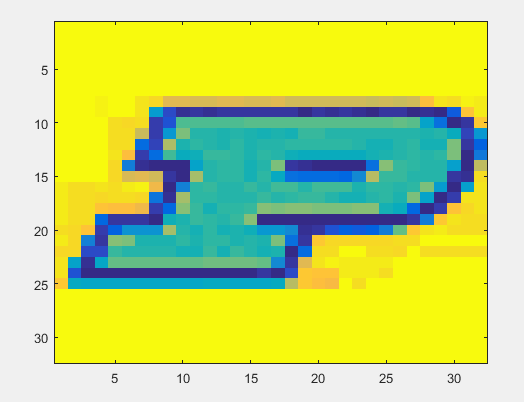
\includegraphics[width=8cm]{color}
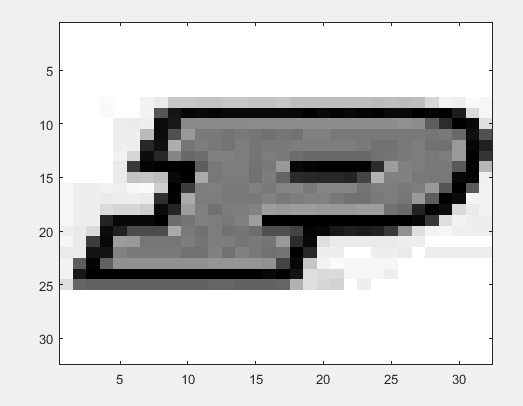
\includegraphics[width=8cm]{gray}
\end{figure}

\item Resahpe command will reshape the input array into a $m\times n$ matrix, and return the new matrix. 


\item Please see the attached code 

\item  This image looks correct, shown as below.  
\begin{figure} [h]
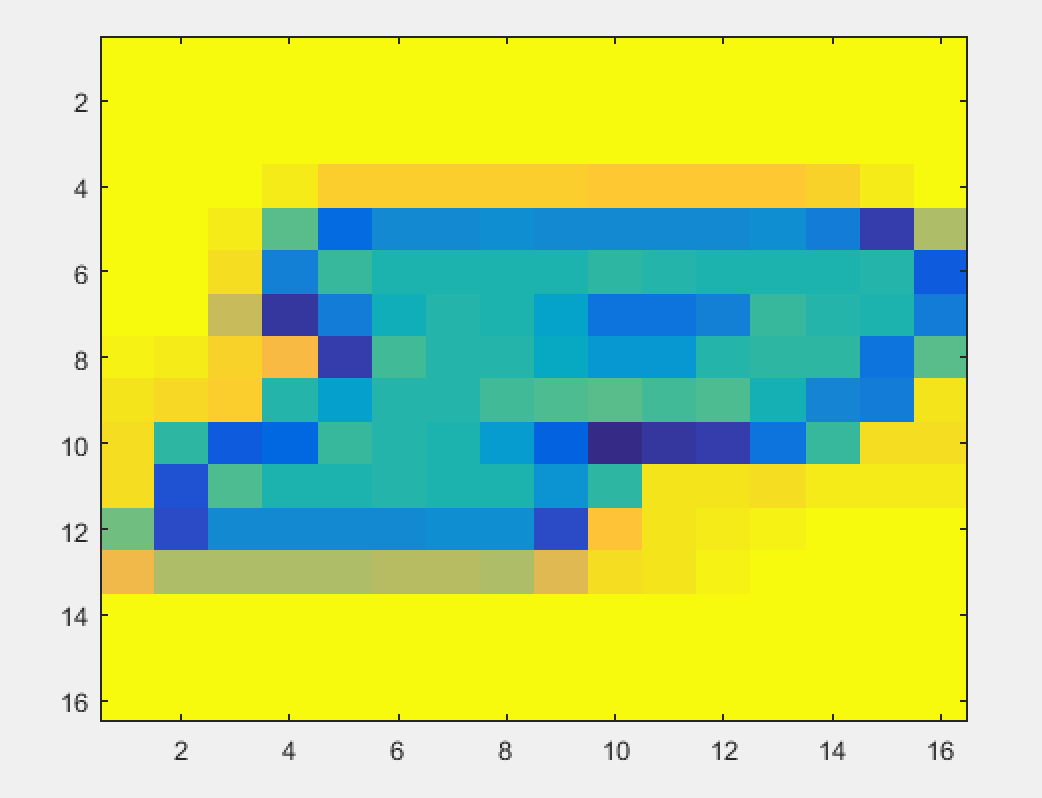
\includegraphics[width=8cm]{reduced}

\end{figure}
It looks correct. 

\item After applying 'interp2' function.  The image would be like this which is very similar with what we got from 
\begin{figure} [h]
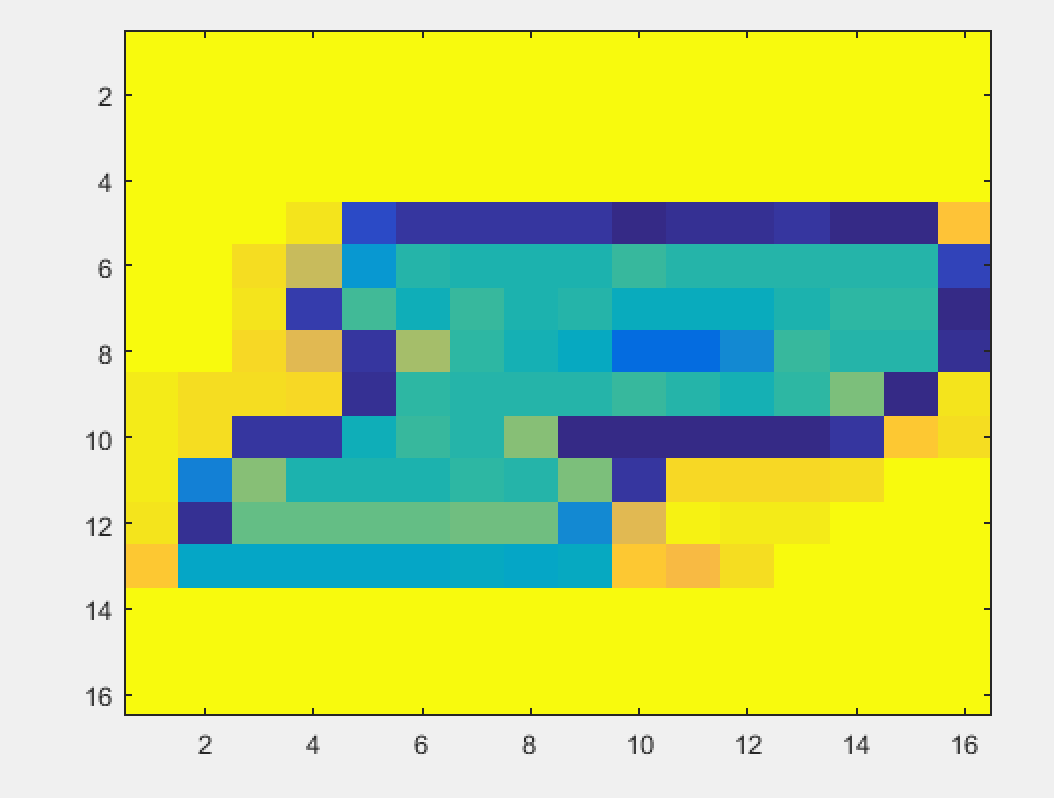
\includegraphics[width=8cm]{interp2}

\end{figure}

\item Here are all the code for Problem 7. 
\begin{lstlisting}
%% Part 2
load smallicon.txt
t = trace(smallicon)
%% Part 3 
imagesc(smallicon)
colormap(gray)
%% Part 4 
%% Part 5
load smallicon.txt
A = zeros(16*16,32*32);    % initialize A matrix
x = zeros(32*32,1);		% initialize B matrix

NX = [32, 1]; % the map between pixel indices and linear indices for X
NY = [16,1]; % the map between pixel indices and linear indices for Y
 for i=1:32
     for j=1:32    
         xi = dot(NX,[i-1,j]); % the index of the pixel i,j in the vector x
         yij = [floor(0.5*i+0.6)-1, floor(0.5*j+0.6)] ; % the resulting location of pixel in the matrix Y
         yi = dot( NY, yij); % the index of the linear pixel in the vector y
         x(xi) = smallicon(i,j);   % fill in the linear vector x
         A(yi,xi) = 1/4; % place the entry of the matrix
     end
   end

  y = A*x;    % Apply matrix on vector x
  Y = reshape(y,16,16)';   % Reshape the linear indexed vector to be an 16 by 16 matrix. 
imagesc(Y)   % Show the downsampled image.  

%% Part 7 

load smallicon.txt
X = smallicon
Ym = interp2(X,-1)
imagesc(Ym) 
\end{lstlisting}

\end{enumerate} 

\end{document} 



